\documentclass[10pt]{article}
\usepackage{fullpage}
\usepackage{amsfonts}
\usepackage{amsmath}
\usepackage{amsthm}
\usepackage{graphicx}
\usepackage{color}
\usepackage{amssymb}
\usepackage{empheq}
\usepackage{mathrsfs}
\usepackage{enumerate}
\usepackage{tikz}
\usepackage{pgflibraryarrows}
\usepackage{pgflibrarysnakes}
\usepackage{upgreek}
\usepackage{tipa}
\usepackage{multicol}
\usepackage{verbatim}
\usepackage{floatrow}
\usepackage{gensymb}
\usepackage{caption}

\usepackage{versions}
\excludeversion{sol}
\includeversion{sol}
\newenvironment{solution}{
\sol\\{\sc{Solution:}}}{
$\hfill\blacksquare$\endsol}

\def\|{||}
\def\R{\textbf{R}}
\def\C{\mathbb{C}}


\usepackage[T1]{fontenc}
\usepackage[font=small,labelfont=bf,tableposition=top]{caption}

\DeclareCaptionLabelFormat{andtable}{#1~#2  \&  \tablename~\thetable}

\newcommand{\pd}[2]{\frac{\partial #1}{\partial #2}}
\newcommand{\pdd}[2]{\frac{\partial^2 #1}{\partial {#2}^2}}
\newcommand{\pddd}[2]{\frac{\partial^3 #1}{\partial {#2}^3}}
\newcommand{\de}[2]{\frac{d #1}{d #2}}
\newcommand{\ppdd}[3]{\frac{\partial^2 #1}{\partial #2 \partial #3}}

\newtheorem*{1}{Problem 1}
\newtheorem*{2}{Problem 2}
\newtheorem*{3}{Problem 3}
\newtheorem*{4}{Problem 4}


\newfloatcommand{capbtabbox}{table}[][\FBwidth]

\usepackage{fancyhdr}
\setlength{\headheight}{15.2pt}
\pagestyle{fancy}
\setlength\headsep{30pt}
\lhead{P4.WS2}
\rhead{Kutztown University -- MATH 210}

\fancyfoot{}


%\rfoot{\tiny\textcopyright \textcolor{gray}{Brooks Emerick}}

\begin{document}

\begin{center}
\Large{\textsc{Phase 4 (part 2): First-Order Systems of ODEs}}\\
\end{center}




%%%%%%%%%%%%%%%%%%%%%%%%%%%%%%%%%%%%%%%%%


\begin{enumerate}[{$\qquad 1.]$}]
\item In pharmaco-kinetics, ``flow of medication'' problems can be easily formulated to track the progression of a drug from the intestine to the bloodstream.  This is called a \textit{compartment-based model}:  
\begin{enumerate}
\item Model the absorption of an antihistamine when ingested into the GI-Tract using the following diagram:
\begin{center}
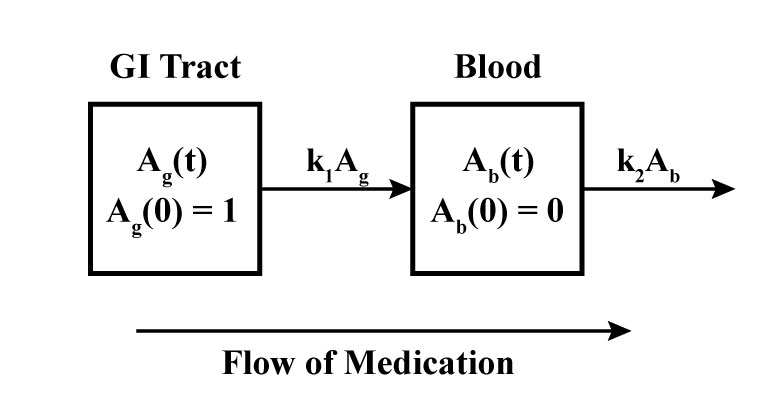
\includegraphics[width = .5\textwidth]{Pharma_3_web.jpg}
\end{center}

Write down the corresponding differential equation system corresponding to this model.  Solve the system in Python and plot both solutions for $A_g(t)$ and $A_b(t)$ on the same figure being sure to label your figure with titles and axes appropriately. Note, $k_1$ and $k_2$ are parameters who values are up to you to decide, but to get started, define $k_1 = 0.6931$ and $k_2 = 0.0231$.  What happens when you change these values? \vfill


\item Suppose there is an influx of medication every 6 hours into the GI Tract.  In this scenario, there is a pulse of medication given by the function $I(t)$:
\begin{center}
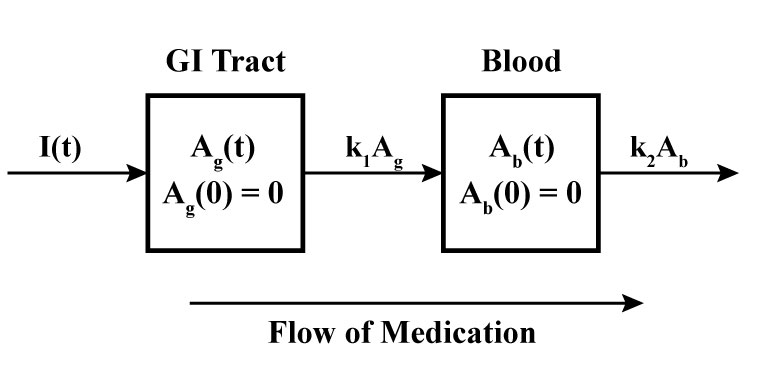
\includegraphics[width = .5\textwidth]{Impulse_Pharma_web.jpg}
\end{center}
Write down the corresponding differential equation system corresponding to this model.  Plot both solutions for $A_g(t)$ and $A_b(t)$ on the same figure being sure to label your figure with titles and axes appropriately.  Define the function $I(t)$ using the mod function in Python to simulate a dosage every 6 hours. \vfill


%\item Repeat part $a.)$, but assume there are 5 compartments in your model.  Instead of just the GI-Tract and the Bloodstream, define five functions $A_i(t)$ for $i = 1, 2, \ldots, 5$ and solve the five equations with parameters $k_i$, for $i = 1,2, \ldots , 5.$  Plot all the solutions on the same graph over time.  Experiment with different values of your parameters to see how the solutions change.

\end{enumerate}

\pagebreak 

\item The Lotka-Volterra equations describe a \textit{predator-prey} relationship: 

\begin{align*}
\frac{dx}{dt} & = \alpha x - \beta xy \\ 
\frac{dy}{dt} & = -\gamma y + \delta xy \end{align*}

Choose a set of parameters for this model and solve the system in Python.  Plot the solutions against time.  Make a second plot that plots $y$ versus $x$. This is called the \textit{Phase Plane}.  Can you describe the relationship between the time series plot and the phase plot? \vfill
  
\item Below is a two-dimensional first-order system of equations that models \textit{competing species}: 

\begin{align*}
\frac{dx}{dt} & = k_1 x \left( 1 - \frac{x}{m_1} \right) - \delta_1 xy \\ 
\frac{dy}{dt} & = k_2 y \left( 1 - \frac{y}{m_2} \right) - \delta_2 xy \end{align*}

Choose a set of parameters for this model and solve the system in Python.  Plot the solutions against time.  Make a second plot that plots $y$ versus $x$.  \vfill
  

\end{enumerate}

















\end{document}